\chapter{Implementierung}
\label{implementierung}
In diesem Kapitel werden wichtige Aspekte bei der Implementierung des Systems aufgezeigt. Auf essentielle Quelltextausschnitte, welche für eine Gewährleistung, der aus den Anforderungen resultierenden Funktionalität verantwortlich sind, wird detailliert eingegangen. Dabei werden wichtige Konzepte, Strukturen und Designentscheidungen der entwickelten Architektur hervorgehoben und aufgetretene Probleme beim Implementierungsprozess dargelegt. Außerdem werden ausgewählte Subsysteme von \texttt{SimpliFX} mit geeigneten Darstellungsmitteln präsentiert und, für ein besseres Verständnis der zusammenarbeitenden Komponenten, eine beispielhafte Nutzung dieser durchgeführt. Die Verwendung und das Zusammenspiel der zuvor in \autoref{annotations} definierten Annotationen, werden durch Quelltextbeispiele erklärt. Dazu werden mögliche mit einhergehende Restriktionen beleuchtet.
\section{Architektur und Struktur der Software}
\label{architektur}
Für die Implementierung und um eine, nach \autoref{nreq3} und \autoref{nreq4}, hohe Softwarequalität sowie Erweiterbarkeit, muss das System durch eine wohlüberlegte Architektur repräsentiert werden. Um eine hohe Unabhängigkeit des Systems zu gewährleisten und eine Überladung mit unnötigen Funktion zu vermeiden, wurde auf die Nutzung von externen Bibliotheken zur Vereinfachung des Implementierungsprozesses und die Reduktion des Zeitaufwandes weitgehend verzichtet. Nur externe Bibliotheken, welche komplexe Funktionen zur Verfügung stellen und daher nicht im Rahmen dieser Arbeit implementiert werden können, sind im Projekt enthalten. Auch dürfen Bibliotheken, welche eine Inkompatibilität mit der im Projekt genutzten Softwarelizenz aufweisen, nicht als Abhängigkeit genutzt werden. Für die Verwaltung der externen Bibliotheken und die Strukturierung des Systems wird, wie in \autoref{konzept_und_modellierung_designentscheidungen} erläutert, das Apache Maven\footref{ft:maven} Build-Management-Tool verwendet. Das Projekt wird nach der finalisierten Implementierung als Maven-Artefakt öffentlich zugänglich und aufgrund der quelloffenen Natur auch per GitHub einsehbar sein. \texttt{SimpliFX} bietet dem Nutzer dazu auch verschiedene spezialisierte Artefakte an, welche an ein bestimmtes Framework für die Abhängigkeitsinjektion angepasst wurde. Für die interne Trennung der Belange und Funktionen von \texttt{SimpliFX}, werden Java Pakete verwendet. Diese Paketstruktur wird im nachfolgenden Unterkapitel näher erläutert. Dabei wird auf die Funktionalität der, in den einzelnen Paketen definierten, Klassen eingegangen und mögliche wichtige Funktionen, Methoden und Klassen mit Beispielen und ausgewählten Quelltextausschnitten vorgestellt und explizit angegeben, ob eventuelle Restriktionen bei der Nutzung zu beachten sind.
\section{Paketstrukturierung nach Funktionalität}
Die verschiedenen Pakete von \texttt{SimpliFX} sind in \autoref{fig:package_structure} dargestellt. Rot markierte Pakete dienen zur Abhängigkeitsinjektion und sind nicht im normalen Funktionsumfang enthalten, sondern nur mittels spezialisierter Maven Artefakte nutzbar. 
\def\Size{4pt}
\definecolor{folderbackground}{RGB}{135,147,154}
\tikzset{
  folder/.pic={
    \filldraw[draw=folderbackground,top color=folderbackground!50,bottom color=folderbackground]
      (-1.05*\Size,0.2\Size+5pt) rectangle ++(.75*\Size,-0.2\Size-5pt);  
    \filldraw[draw=folderbackground,top color=folderbackground!50,bottom color=folderbackground]
      (-1.15*\Size,-0.7*\Size) rectangle (1.15*\Size,\Size);
  },
  folderopt/.pic={
    \filldraw[draw=red,top color=red!50,bottom color=red]
      (-1.05*\Size,0.2\Size+5pt) rectangle ++(.75*\Size,-0.2\Size-5pt);  
    \filldraw[draw=red,top color=red!50,bottom color=red]
      (-1.15*\Size,-0.7*\Size) rectangle (1.15*\Size,\Size);
  }
}
\begin{figure}[H]
	\centering
	\begin{forest}
		for tree={
			font=\ttfamily,
			grow'=0,
			child anchor=west,
			parent anchor=south,
			anchor=west,
			inner xsep=8pt,
			inner ysep=0pt,
			if n=5{edge path={\noexpand\path [draw, \forestoption{edge}] (!u.south west)+(12.5pt,0) |- (.child anchor) pic {folderopt}\forestoption{edge label};}}{if n={11}{edge path={\noexpand\path [draw, \forestoption{edge}] (!u.south west)+(12.5pt,0) |- (.child anchor) pic {folderopt}\forestoption{edge label};}}{if n={15}{edge path={\noexpand\path [draw, \forestoption{edge}] (!u.south west)+(12.5pt,0) |- (.child anchor) pic {folderopt}\forestoption{edge label};}}{edge path={\noexpand\path [draw, \forestoption{edge}] (!u.south west)+(12.5pt,0) |- (.child anchor) pic {folder}\forestoption{edge label};}}}},
			if n children=0{}{
				delay={
					prepend={[,phantom, calign with current]}
				}
			},
			fit=band,
			before computing xy={l=35pt}
		}
		[de.intelligence.bachelorarbeit.simplifx
			[annotation]
			[application]
			[classpath]
			[css]
			[dagger1]
			[di]
			[event]
			[events]
			[exception]
			[fxml]
			[guice]
			[injection]
			[localization]
			[logging]
			[spring]
			[utils]
		]
	\end{forest}
	\caption{Paketstruktur -- \texttt{SimpliFX}}
	\label{fig:package_structure}
\end{figure}
\subsubsection{Paket: utils}
Das \texttt{utils} Paket beinhaltet Klassen und Methoden, welche häufig genutzte Operationen an zentraler Stelle kombiniert. Außerdem werden Werkzeugklassen bereitgestellt, die in der Form nicht im Funktionsumfang von Java enthalten sind. Dazu gehören beispielsweise funktionale Schnittstellen mit einer Unterstützung von Ausnahmen, Klassen für das Überprüfen von Nullbarkeit oder bool'schen Bedingungen und Implementierungen der \texttt{Iterator} Schnittstelle, welche durch das Nutzen von \texttt{AutoCloseable}, Ressourcen schließen kann und damit eine Prävention von eventuellen Ressourcenlecks gewährleistet. Die Klasse \texttt{CloseableWrappedIterator}, erlaubt das Erstellen einer \texttt{Iterator} Instanz, welche bei Nutzung der \texttt{stream} Methode, alle genutzten Ressourcen bei einem Ende des Streams automatisch schließt. Außerdem wurde die Funktionalität der \texttt{Map.Entry} Klasse in die \texttt{Pair} Klasse ausgelagert, von welcher eine beispielhafte Nutzung in \autoref{lst:pair} dargestellt ist.
\begin{figure}[H]
	\begin{lstlisting}[caption=Beispiel -- Nutzung der \texttt{Pair} Klasse., captionpos=b, label=lst:pair]
final Pair<String, Integer> pair = Pair.of("test", 0);
System.out.println(pair.getLeft()); // test
System.out.println(pair.getRight()); // 0
	\end{lstlisting}
\end{figure}
\subsubsection{Paket: di}
Schnittstellen für die Unterstützung von Abhängigkeitsinjektion, werden durch das \texttt{di} Paket bereitgestellt. Die eigentliche Implementierung dieser Schnittstellen, ist in externen  Artefakten zu finden, auf welche in den folgenden drei Untersektionen näher eingegangen wird.
Das Paket stellt zwei Klassen, \texttt{DIEnvironment} und \texttt{IDIEnvironmentFactory} sowie die \texttt{@DIAnnotation} zur Verfügung. Wenn eine weitere Bibliothek zur Laufzeitinjektion von Abhängigkeiten genutzt werden soll, welche nicht im Funktionsumfang von \texttt{SimpliFX} enthalten sind, müssen Implementationen für beide Schnittstellen, sowie eine Annotation für die jeweilige Bibliothek bereitgestellt werden.
\begin{figure}[H]
	\centering
	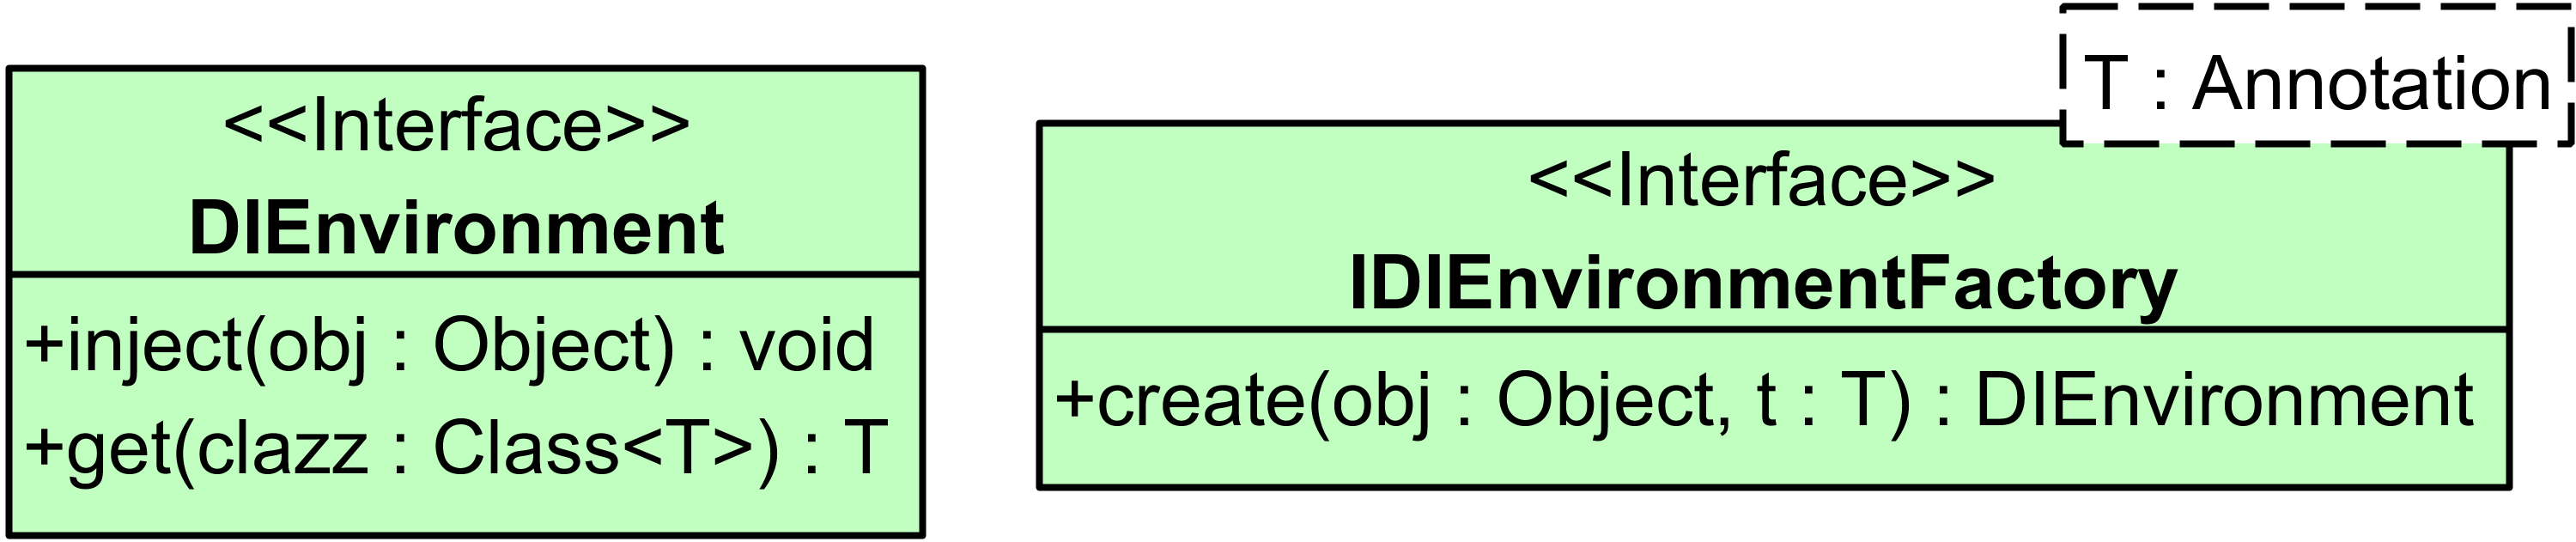
\includegraphics[width=\textwidth-2cm]{Abbildungen/DI Paket.png}
	\caption{Diagramm -- DI Schnittstellen.}
	\label{fig:di_package}
\end{figure}
\noindent \texttt{SimpliFX} kennt die Implementierung der in \autoref{fig:di_package} dargestellten Klassen nicht und kann daher mit Leichtigkeit um weitere Bibliotheken zur Abhängigkeitsinjektion erweitert werden. Zuerst muss der Entwickler eine Implementierung der \texttt{DIEnvironment} Klasse erstellen, welche für das Injizieren von vorhandenen Objekten und das Instanziieren von neuen Objekten verantwortlich ist. Danach muss eine \texttt{IDIEnvironmentFactory} mit dem Typen der Annotation als generischen Parameter erstellt werden, welche den alleinigen Zweck hat, neue Instanzen der vorher erstellten \texttt{DIEnvironment} Implementierung zu generieren. Letztlich muss der Entwickler eine Laufzeitannotation erstellen, welche an Typdefinitionen angebracht werden kann und dazu die Meta-Annotation \texttt{@DIAnnotation} mit der jeweiligen Implementierungsklasse der \texttt{IDIEnvironmentFactory} Schnittstelle als Parameter aufweist. Das Registrieren einer neuen Bibliothek ist in \autoref{appendix:add_new_di_library} gezeigt.
\subsubsection{Paket: dagger1}
Das \texttt{dagger1} Paket ist für die Integration von Dagger 1\footnote{Dagger 2 realisiert Abhängigkeitsinjektion ausschließlich zur Kompilierzeit, weshalb Schnittstellen zum reflektiven injizieren von Abhängigkeiten wie den \texttt{ObjectGraph} nicht mehr existieren und somit ein Zugang von \texttt{SimpliFX} auf den Injizierungsprozess ausgeschlossen ist.} in \texttt{SimpliFX} zuständig. Die \texttt{Dagger1Environment} Klasse definiert eine neue \texttt{ObjectGraph} Instanz aus den übergebenen Modulobjekten, welche für die Injektion verantwortlich ist. Dabei kann die Methode \texttt{ObjectGraph\#inject} genutzt werden, um Abhängigkeiten in eine vorhandene Instanz zu injizieren und \texttt{ObjectGraph\#get} um eine neue Klasseninstanz zu erstellen. 
\subsubsection{Paket: guice}
Das \texttt{guice} Paket ist für die Integration von Guice in \texttt{SimpliFX} zuständig. Dabei wird von der \texttt{GuiceEnvironment} Klasse ein neuer \texttt{Injector} erstellt, welcher durch die Methode \texttt{Injector\#injectMembers} Abhängigkeiten injiziert und mit \texttt{Injector\#getInstance} neue Instanzen erstellt.
\subsubsection{Paket: spring}
Das \texttt{spring} Paket ist für die Integration von Spring in \texttt{SimpliFX} zuständig.
Die Umgebungsklasse für Spring (\texttt{SpringEnvironment}) erstellt eine neue Instanz der \texttt{AnnotationConfigApplicationContext} Klasse, welche es ermöglicht, mittels einer \texttt{AutowireCapableBeanFactory}, Abhängigkeiten in bestehende Instanzen zu injizieren, sowie neue Instanzen aus Klassen zu erstellen.
\subsubsection{Paket: localization}
\subsubsection{Paket: exception}
\subsubsection{Paket: injection}
\subsubsection{Paket: css}
\subsubsection{Paket: classpath}
\subsubsection{Paket: event}
Das Event System findet seinen Ursprung im \texttt{event} Paket. Es setzt sich aus einer Schnittstelle, deren Implementierung und der \texttt{@EventHandler} Annotation zusammen. Die \texttt{IEventEmitter} Klasse (siehe \autoref{fig:event_emitter}) ermöglicht das Registrieren sowie das Abmelden eines Objektes beim System. Bei der Registrierung wird das übergebene Objekt auf Methoden untersucht, welche mit \texttt{@EventHandler} annotiert wurden, validiert diese und speichert sie in einem internen Methoden Cache. Die Validierung ist nötig, da gefundene Methoden nur exakt einen Parameter als Event aufweisen dürfen. 
\begin{figure}[H]
	\centering
	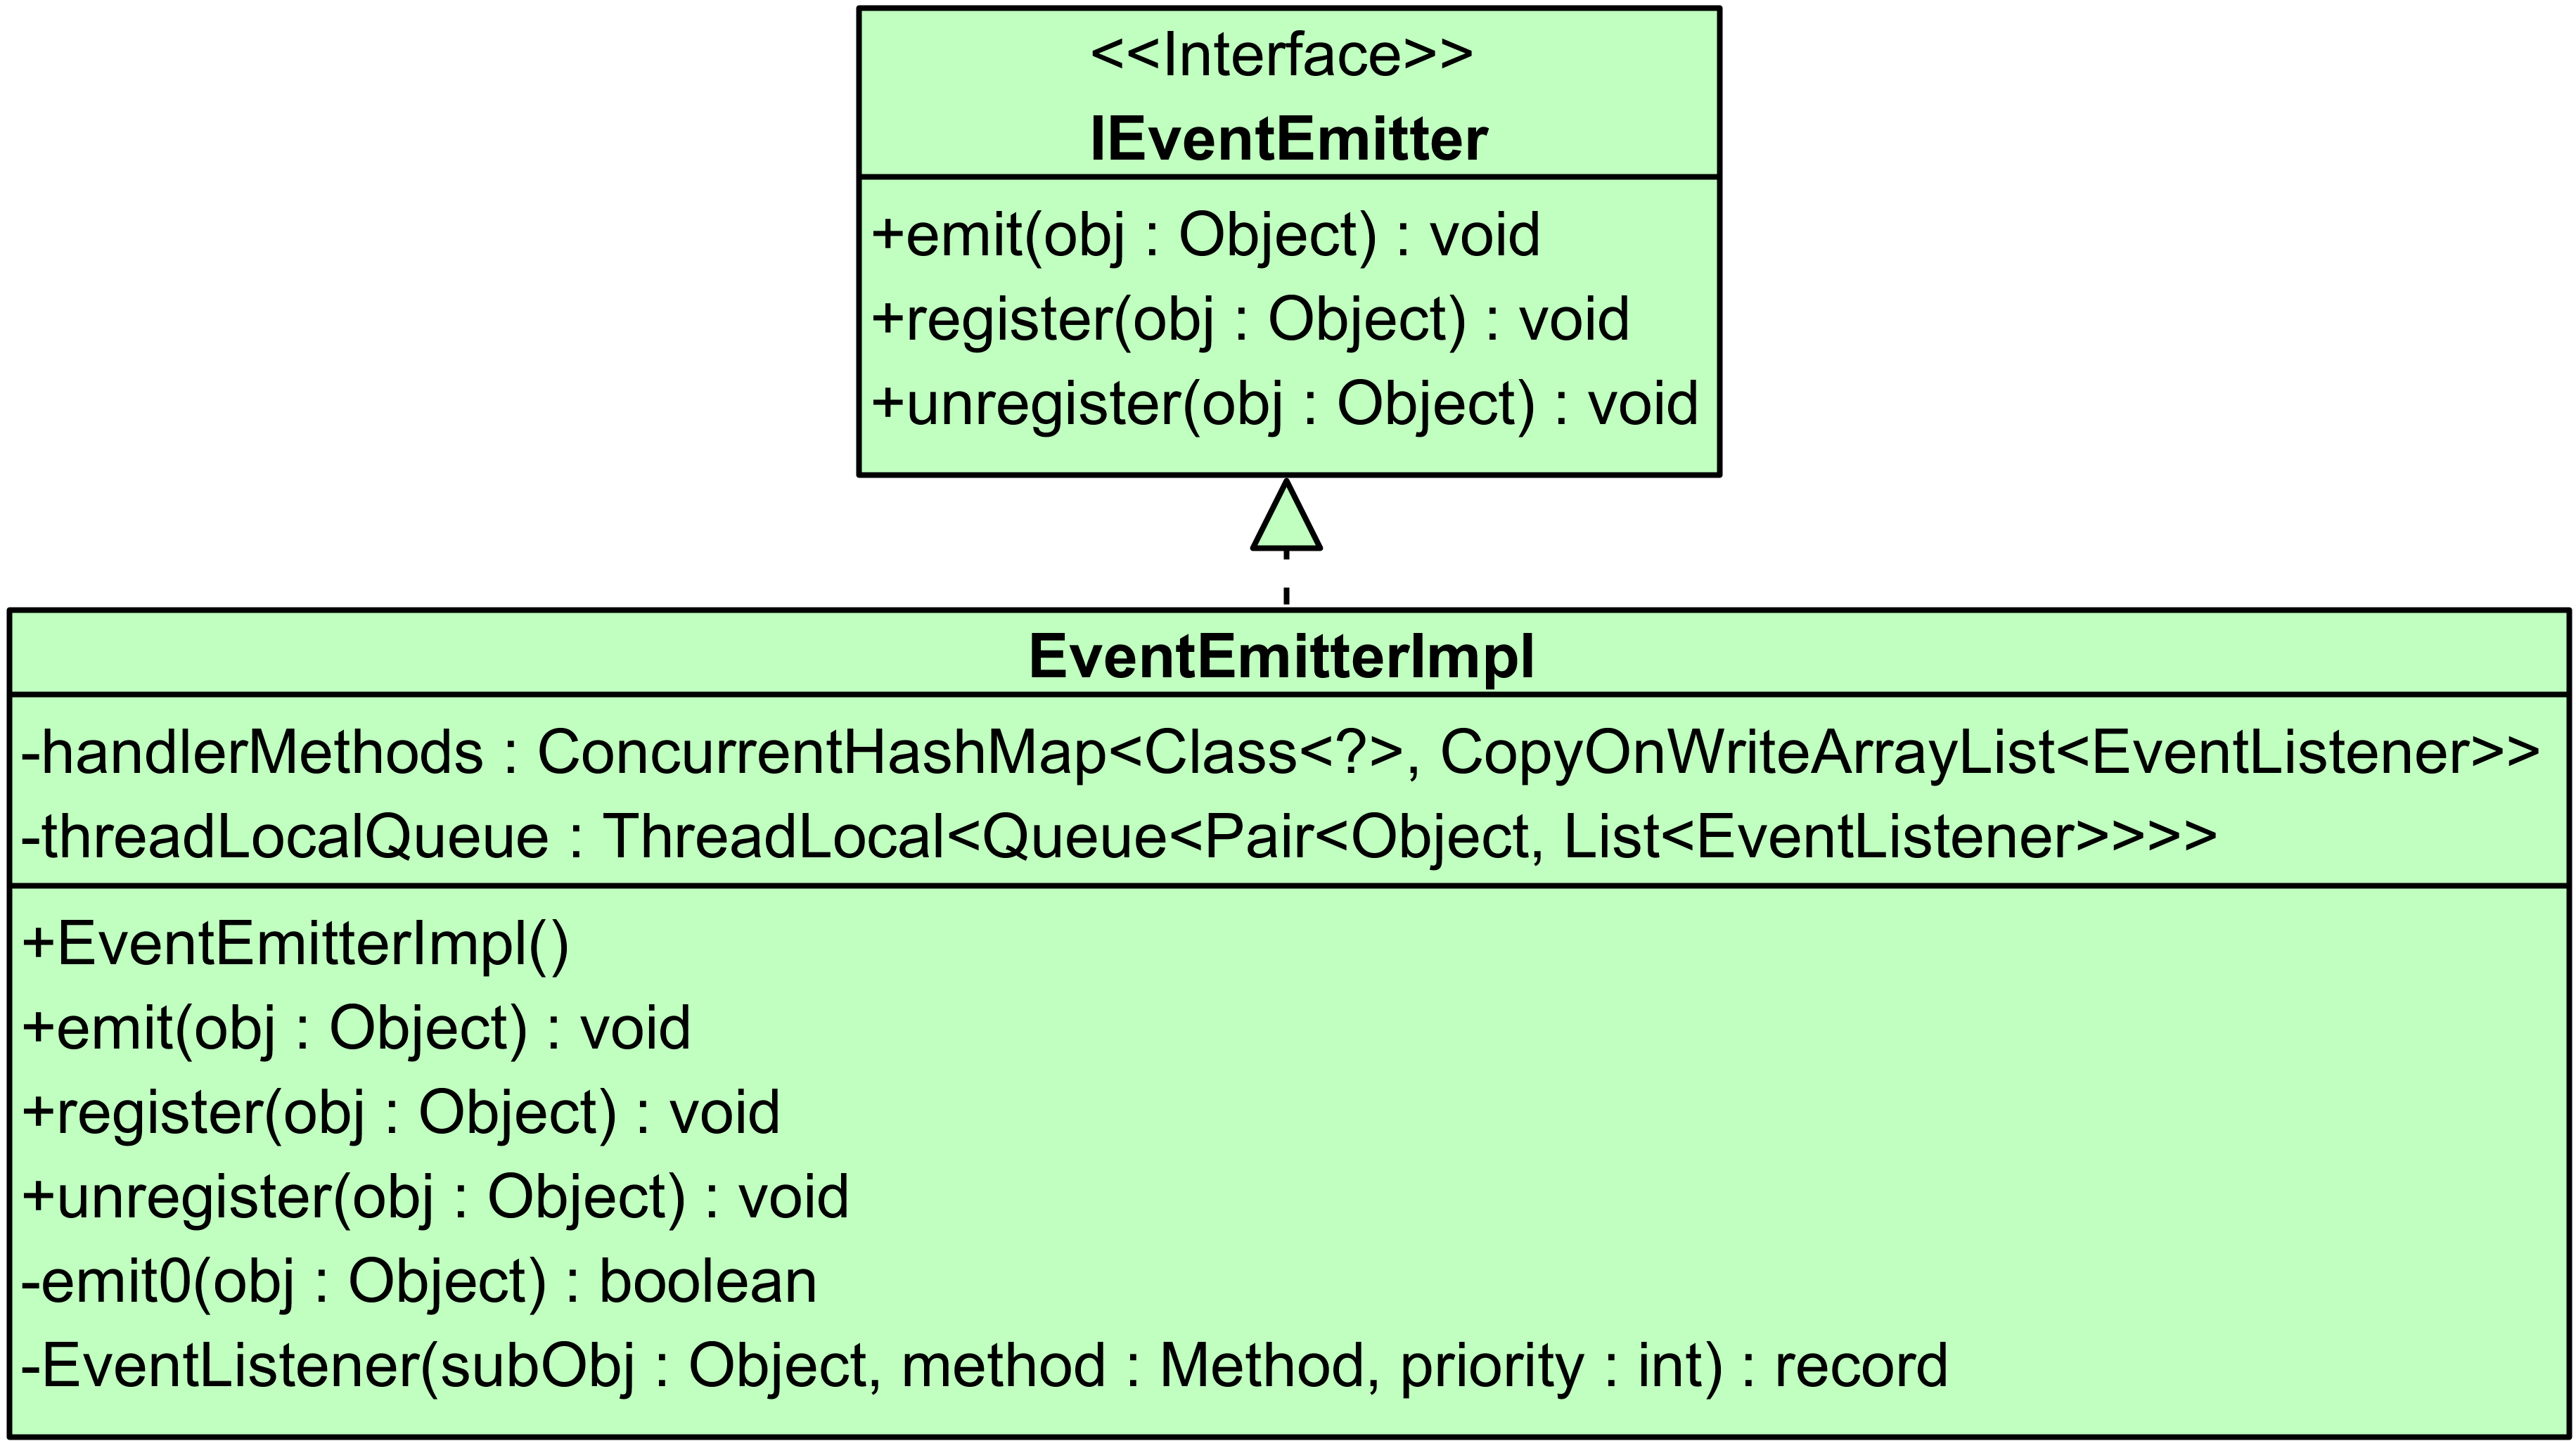
\includegraphics[width=\textwidth-4cm]{Abbildungen/EventEmitter.png}
	\caption{Diagramm -- IEventEmitter Schnittstelle und Implementierung.}
	\label{fig:event_emitter}
\end{figure}
\noindent Mit der \texttt{IEventEmitter\#emit} Methode, wird dem System ein neues Event übermittelt und alle Methoden welche für dieses Event registriert wurden, nach Priorität der Annotation aufgerufen. Die daraus resultierenden Methodenaufrufe werden dabei auf dem aufrufenden \texttt{Thread} ausgeführt und blockieren diesen, bis alle Aufrufe abgeschlossen wurden.
\subsubsection{Paket: events}
Das \texttt{events} Paket stellt eine Vielzahl an Standard-Events für beispielsweise den Lebenszyklus der Applikation (\texttt{InitEvent}, \texttt{StartEvent}, \texttt{StopEvent}) oder für Statusaktualisierungen des Preloaders (\texttt{StateChangeEvent}, \texttt{ProgressEvent}) bereit. Diese können durch eine \texttt{IEventEmitter} genutzt werden.
\subsubsection{Paket: application}
Die von \texttt{SimpliFX} verwalteten JavaFX Applikation- und Preloader-Klassen sowie die dafür benötigten Annotation sind im \texttt{application} Paket enthalten und definieren alle Methoden, welche durch die Applikation- respektive Preloaderklasse vererbt werden (siehe \autoref{fig:app_package}). Dabei wird bei der Erstellung der Klassen, eine für den Typ des Einstiegspunktes spezifische \texttt{IEventEmitter} Instanz übergeben, welche etwaige interne Methodenaufrufe in Form von vordefinierten Events an den vom Entwickler definierten, Einstiegspunkt delegiert.
\begin{figure}[H]
	\centering
	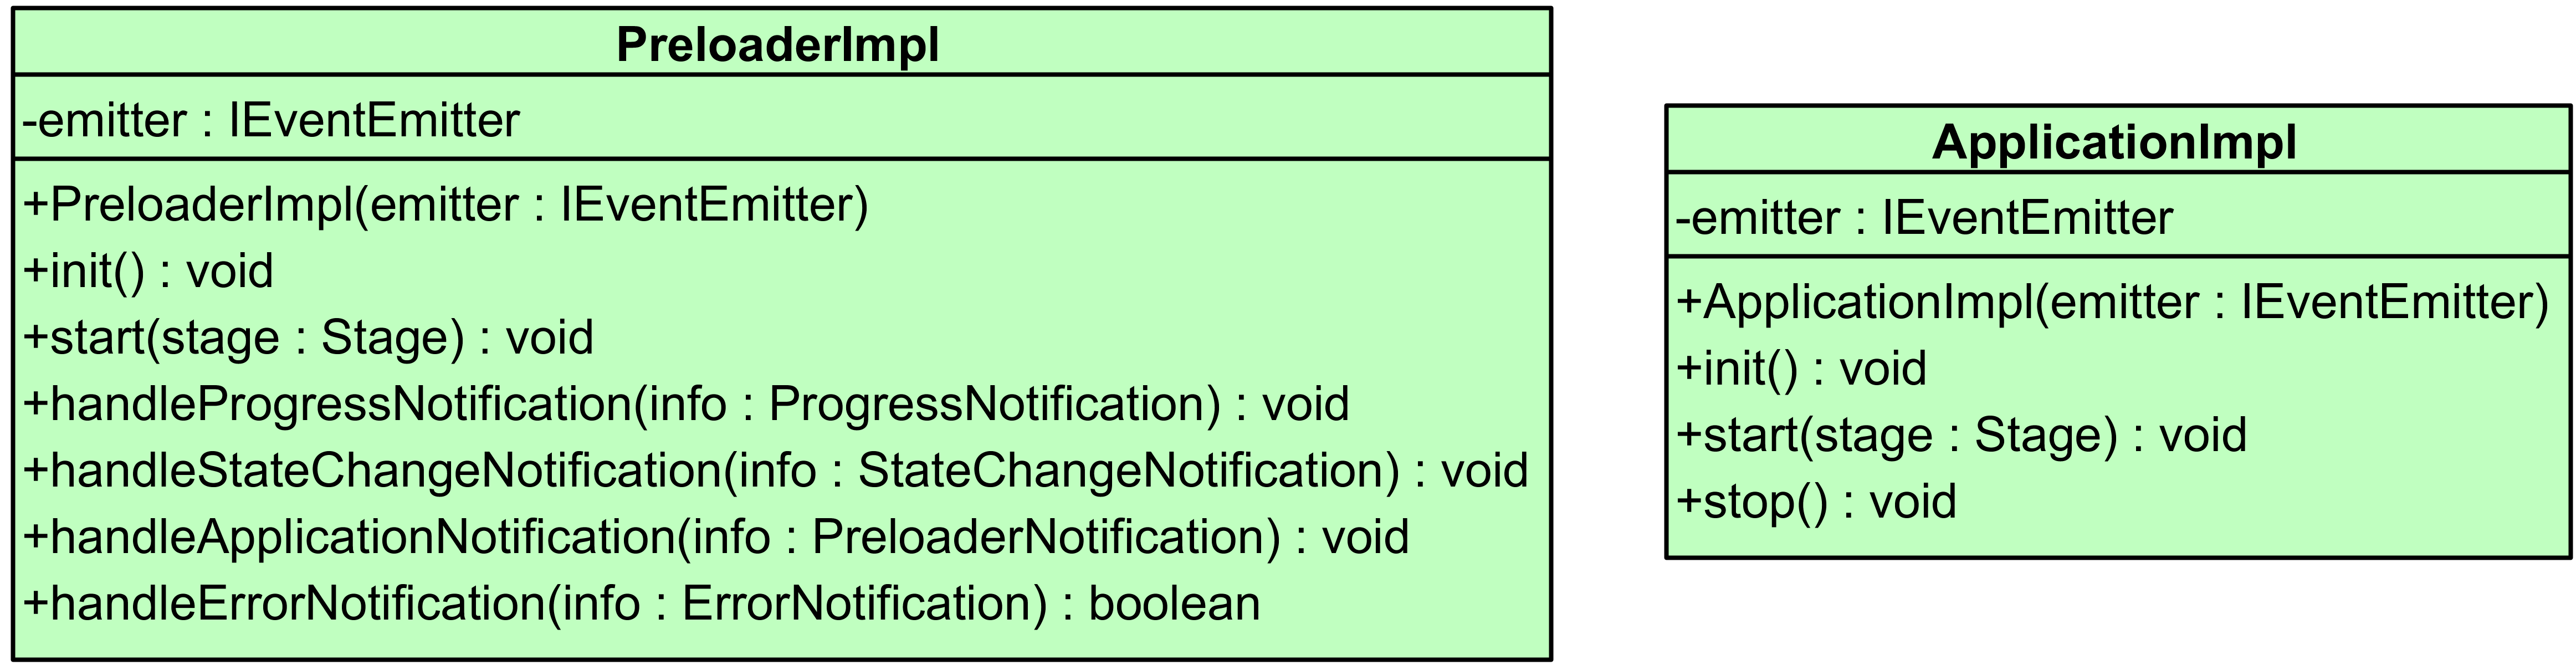
\includegraphics[width=\textwidth-2cm]{Abbildungen/Applikation und Preloader.png}
	\caption{Diagramm -- Applikation und Preloader.}
	\label{fig:app_package}
\end{figure}